\chapter{Organización del código}

\#NOTA: Las clases tanto de desarrolo backend y frontend hacen match entre sus atributos y sus clases de respuesta y solicitud.
\section{Spring}

\begin{figure}[H]
    \centering
    
\includegraphics[width=0.4\linewidth]{images/tecnologias/spring.png}
\end{figure}

Para el desarrollo de backend, se utilizó el framework Spring, el cual por defecto nos ofrece un patrón de arquitectura de software Modelo-Vista-Controlador.

\subsection{Entidades}
Para llevar a cabo la programación, se usó una implementación donde cada entidad tiene su propio folder el cual contiene 4 archivos principales:

\begin{itemize}
    \item Entidad.java
    \item EntidadRepository.java
    \item EntidadService.java
    \item EntidadRestController.java
\end{itemize}

\subsection{Entidad.java}
Este archivo de java, es la clase de la endiad la cual contiene toda la información abstraída de la entidad, esto es, sus atributos, sus relaciones con otras entidades, sus llaves primarias y sus restricciones.
\subsection{EntidadRepository.java}
Este archivo de java es una clase donde se encuentran todas aquellas consultas que se realizaran a la base de datos.
Al usar spring, nos da la fácilidad de utilziar diferentes gestores de entidades, en este sistema se utilizó la libreria de JPA, la cual nos ofrecé las consultas más básicas que puedes hacer a una bae de datos.
También, esta clase nos ayuda a hacer las consultas que son más especificas, por ejemplo, consultar entidades por una relación con otra.
\subsection{EntidadService.java}
Este archivo de java, es una clase que organiza las consultas creadas en la clase Repository, es un gran cátalogo de las consultas.
\subsection{EntidadRestController.java}
Este archivo de java, es la clase en la que encuentra la lógica de programación, el que distribuye las consultas de http y ejecuta distintas funciones dependiendo de cual es la petición relizada.
Ésta vista es la puerta de acceso al mundo exterior, quien recibe peticiones hechas por el usuario al sistema, procesa la información solicitada y envia una respuesta al usuario.

La respuesta que manda esta definida en una clase y se describe en la siguiente imagen:
%\begin{figure}[H]
	%\centering
	%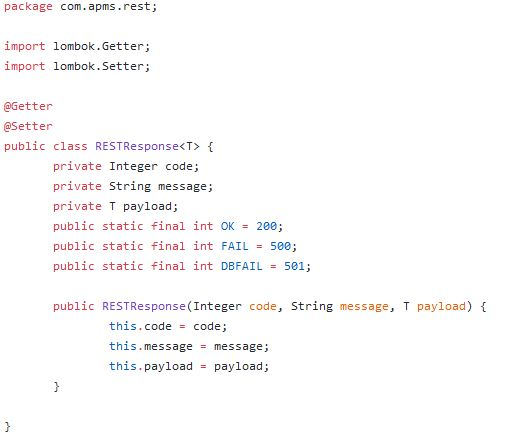
\includegraphics[width=0.6\linewidth]{images/tecnologias/Response}
%	\caption{Representación gráfica del objeto de respuesta que se manda a través de spring hacía el usuario.}
%\end{figure}
Esta clase tiene definido las 3 tipos de respuesta que puede regresar el sevidor:
\begin{itemize}
    \item OK: Para respuestas donde la información se proceso de manera correcta.
    \item FAIL: Para respuestas donde hubo algun error al momento de procesar la petición.
    \item DBFIAL: Error en la base de datos.
\end{itemize}
Y dentro de sus atributos tiene definidos 3:
\begin{itemize}
    \item code: Es el tipo de respuesta que regresa el servidor.
    \item message: Un mensaje que regresa el servidor para saber que es lo que pasó.
    \item payload: Información de la respuesta generada.
\end{itemize}

\subsection{Angular}



\begin{figure}[H]
    \centering
    
\includegraphics[width=0.4\linewidth]{images/tecnologias/angular.png}
\end{figure}